\documentclass[aspectratio=169]{beamer}
\mode<presentation>
{
  \usetheme{metropolis}      % or try Darmstadt, Madrid, Warsaw, ...
  \usecolortheme{default} % or try albatross, beaver, crane, ...
  \usefonttheme{structurebold}  % or try serif, structurebold, ...
  \setbeamercolor{background canvas}{bg=white}
  \setbeamertemplate{navigation symbols}{}
  \setbeamertemplate{bibliography item}{\insertbiblabel}
  %\setbeamertemplate{caption}[numbered]
} 
\usepackage[english]{babel}
\usepackage[utf8x]{inputenc}
\usepackage{listings}             % Include the listings-package
\hypersetup{
    colorlinks = true,
    linkcolor = {black},
    urlcolor = {blue}
}
\usepackage{animate}

\DeclareMathOperator*{\argmin}{arg\,min}

\title[Deep Learning and Temporal Data Processing]{Deep Learning and Temporal Data Processing}
\subtitle{Introduction to TensorFlow}
\institute{University of Modena and Reggio Emilia}
\author{Andrea Palazzi}
%\date{June 21th, 2017}

\def\thisframelogos{}

\newcommand{\framelogo}[1]{\def\thisframelogos{#1}}

\addtobeamertemplate{frametitle}{}{%
\begin{tikzpicture}[remember picture,overlay]
\node[anchor=north east] at (current page.north east) {%
    \foreach \img in \thisframelogos {%
        %\hspace{.5ex}%
        \includegraphics[height=3.5ex]{\img}%
    }%
};
\end{tikzpicture}}

\begin{document}

\framelogo{img/template/logo_unimore_white.png}

\bgroup
\renewcommand{\insertframenumber}{}
\begin{frame}[noframenumbering]
  \titlepage
\end{frame}
\egroup
\begin{frame}{Agenda}
  \tableofcontents
\end{frame}


%%%%%%%%%%%%%%%%%%%%%%%%%%%%%%%%%%%%%%%%%%%%%%%%%%%%%%%%%%%%%%%%%%
%%%%%%%%%%%%%%%%%%%%%%%%%%%%%%%%%%%%%%%%%%%%%%%%%%%%%%%%%%%%%%%%%%
%%%%%%%%%%%%%%%%%%%%%%%%%%%%%%%%%%%%%%%%%%%%%%%%%%%%%%%%%%%%%%%%%%

\section{Purpose}

\begin{frame}{Aim of this tutorial}
This short tutorial aims at providing the very basics of TensorFlow.\\
\vspace{0.5cm}
The goal is to understand \textit{what is} TensorFlow, \textit{why do we need it} for deep learning, and \textit{how does it work} from an high-level perspective.\\
\vspace{0.5cm}
Conversely, the next lectures will be more "hands-on": there we'll see actual code examples and we'll use our TF skills to tackle some easy task.
\end{frame}

%%%%%%%%%%%%%%%%%%%%%%%%%%%%%%%%%%%%%%%%%%%%%%%%%%%%%%%%%%%%%%%%%%
%%%%%%%%%%%%%%%%%%%%%%%%%%%%%%%%%%%%%%%%%%%%%%%%%%%%%%%%%%%%%%%%%%
%%%%%%%%%%%%%%%%%%%%%%%%%%%%%%%%%%%%%%%%%%%%%%%%%%%%%%%%%%%%%%%%%%

\section{Why TensorFlow}

\begin{frame}{TensorFlow™\cite{tensorflow2015-whitepaper}}
\textbf{Open source software library for numerical computation using data flow graphs.}\\
\vspace{0.5cm}
\begin{figure}
\begin{tabular}{c}
	
\includegraphics[width=0.35\textwidth]{img/tf/tf_logo.png}
\end{tabular}
\end{figure}
\end{frame}

%%%%%%%%%%%%%%%%%%%%%%%%%%%%%%%%%%%%%%%%%%%%%%%%%%%%%%%%%%%%%%%%%%

\begin{frame}{Why TensorFlow}
Why not \textit{Theano} / \textit{Torch} / \textit{Caffe} / \textit{Microsoft Cognitive Toolkit} / $\dots$ ?\\
\vspace{0.5cm}
\begin{columns}
\begin{column}{0.3\textwidth}
\begin{figure}
\begin{tabular}{c}
	
\includegraphics[width=0.9\textwidth]{img/tf/tf_logo.png}
\end{tabular}
\end{figure}
\end{column}
\begin{column}{0.7\textwidth}
	\begin{itemize}
	\item Python API
	\item Flexible enough for research, yet built with production use in mind
	\item Portable on heterogeneous systems, from mobile devices to large-scale distributed machines, and on a variety of OS (Android, Windows, iOS, ...).
	\item TensorBoard visualization has no rival.
	\item Large community and supported by Google.
	\end{itemize}
\end{column}
\end{columns}
\end{frame}

%%%%%%%%%%%%%%%%%%%%%%%%%%%%%%%%%%%%%%%%%%%%%%%%%%%%%%%%%%%%%%%%%%

\begin{frame}{Disclaimer}
There are a variety of good resources and tutorial to learn TensorFlow.\\
\vspace{0.5cm}
However, please keep in mind that TensorFlow is under heavy development and is constantly changing. In case of doubt, always refer to the official site: \url{https://www.tensorflow.org}.
\end{frame}

%%%%%%%%%%%%%%%%%%%%%%%%%%%%%%%%%%%%%%%%%%%%%%%%%%%%%%%%%%%%%%%%%%
%%%%%%%%%%%%%%%%%%%%%%%%%%%%%%%%%%%%%%%%%%%%%%%%%%%%%%%%%%%%%%%%%%
%%%%%%%%%%%%%%%%%%%%%%%%%%%%%%%%%%%%%%%%%%%%%%%%%%%%%%%%%%%%%%%%%%
%Nodes in the graph represent mathematical operations, while the graph edges represent the multidimensional data arrays (tensors) communicated between them. 

\section{TensorFlow Basics}

\begin{frame}{Computational Graph}
All operations are encapsulated in a computational graph.\\
\vspace{0.5cm}
\textbf{Graph definition is totally separated from execution.}\vspace{0.5cm}
\begin{figure}
\begin{tabular}{c}
	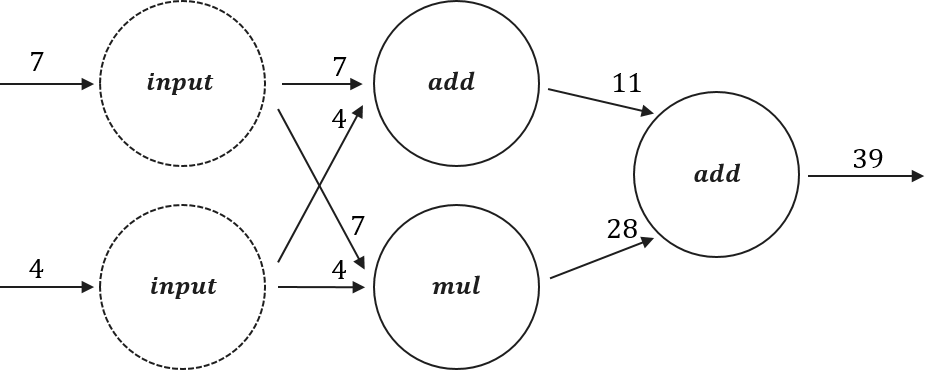
\includegraphics[width=0.7\textwidth]{img/tf/computational_graph.png}
\end{tabular}
\end{figure}
\end{frame}

%%%%%%%%%%%%%%%%%%%%%%%%%%%%%%%%%%%%%%%%%%%%%%%%%%%%%%%%%%%%%%%%%%

\begin{frame}{Graph Definition}
Graph definition is totally separated from execution.\\
\textbf{So what?}
\begin{figure}
\begin{tabular}{c}
	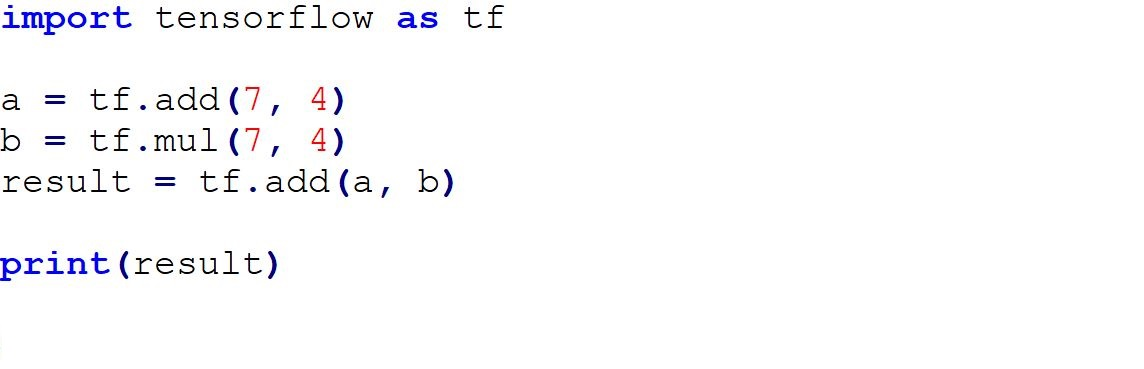
\includegraphics[width=0.9\textwidth]{img/tf/graph_definition_0.jpg}
\end{tabular}
\end{figure}
\end{frame}

%%%%%%%%%%%%%%%%%%%%%%%%%%%%%%%%%%%%%%%%%%%%%%%%%%%%%%%%%%%%%%%%%%

\begin{frame}{Graph Definition}
Graph definition is totally separated from execution.\\
\textbf{So what?}
\begin{figure}
\begin{tabular}{c}
	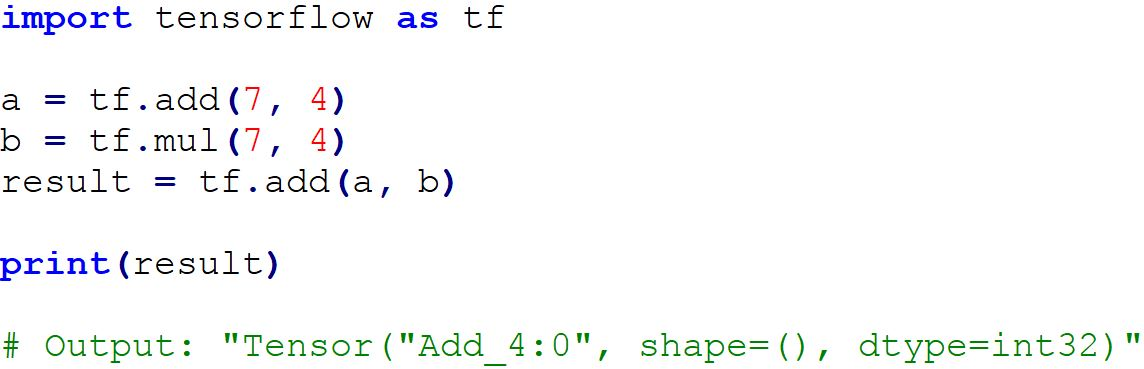
\includegraphics[width=0.9\textwidth]{img/tf/graph_definition_1.jpg}
\end{tabular}
\end{figure}
\textit{What did you expect}? :-)
\end{frame}

%%%%%%%%%%%%%%%%%%%%%%%%%%%%%%%%%%%%%%%%%%%%%%%%%%%%%%%%%%%%%%%%%%

\begin{frame}{Tensors}
In this framework, we can think of \textbf{tensors} as \textbf{n-dimensional matrices}.\\
\vspace{0.25cm}
This allows to abstract over the precise data structure, \textit{e.g.}:
\begin{itemize}
\item[0-d] scalars
\item[1-d] vectors
\item[2-d] matrices
\item[] $\dots$
\end{itemize}
Tensors are represented as the \textbf{edges of the computational graph}.\\
The number of dimensions of a tensor is called \textbf{rank}.
\end{frame}

%%%%%%%%%%%%%%%%%%%%%%%%%%%%%%%%%%%%%%%%%%%%%%%%%%%%%%%%%%%%%%%%%%

\begin{frame}{Graph Evaluation}
In order to get a numerical result we have to \textbf{evaluate the symbolic graph}.\\
\begin{figure}
\begin{tabular}{c}
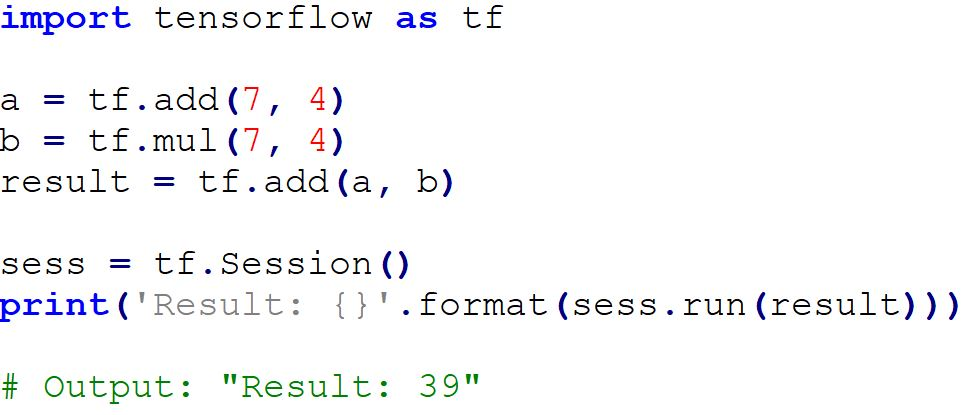
\includegraphics[width=0.75\textwidth]{img/tf/graph_evaluation.jpg}
\end{tabular}
\end{figure}
A \textbf{Session} object encapsulates the environment in which Operation objects are executed, and Tensor objects are evaluated.
\end{frame}

%%%%%%%%%%%%%%%%%%%%%%%%%%%%%%%%%%%%%%%%%%%%%%%%%%%%%%%%%%%%%%%%%%

\begin{frame}{Placeholders}
In order to fed value at execution time, TensorFlow provides a \textbf{placeholder} Operation.\\
\vspace{0.25cm}
Example:
\begin{figure}
\begin{tabular}{c}
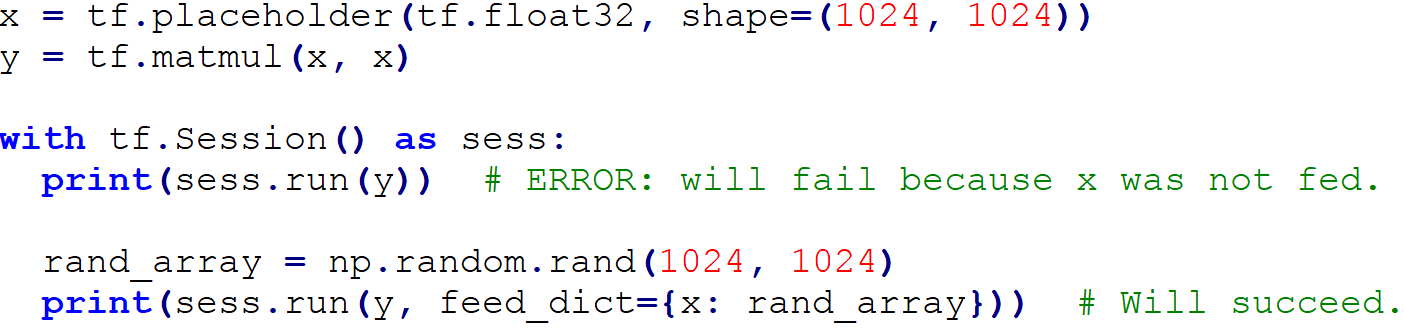
\includegraphics[width=0.95\textwidth]{img/tf/placeholders.png}
\end{tabular}
\end{figure}
Other advanced methods for feeding the computational graph exist, yet these are out of the scope these introductory lectures.
\end{frame}

%%%%%%%%%%%%%%%%%%%%%%%%%%%%%%%%%%%%%%%%%%%%%%%%%%%%%%%%%%%%%%%%%%

\begin{frame}{Variables}
\textbf{Variables} are the core types we want to use when building a machine learning models. Indeed, variables' derivatives can be automatically computed by TensorFlow, which make possible easily implementing \textbf{gradient-based learning} strategies.\\
\vspace{0.5cm}
For this reason, learnable parameters in a machine learning models (\textit{e.g.} weights and biases of a deep network) are implemented as trainable variables.
\begin{figure}
\begin{tabular}{c}
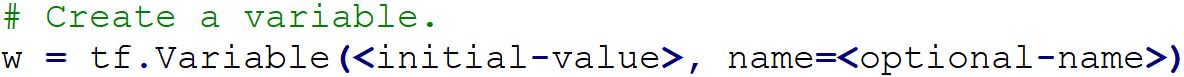
\includegraphics[width=0.8\textwidth]{img/tf/variable_creation.jpg}
\end{tabular}
\end{figure}
\end{frame}

%%%%%%%%%%%%%%%%%%%%%%%%%%%%%%%%%%%%%%%%%%%%%%%%%%%%%%%%%%%%%%%%%%

\begin{frame}{Variable Initialization}
When you launch the graph, \textbf{variables have to be explicitly initialized} before you can run operations that use their value. To this purpose the convenience function \texttt{global\_variables\_initializer} is commonly used.
\begin{figure}
\begin{tabular}{c}
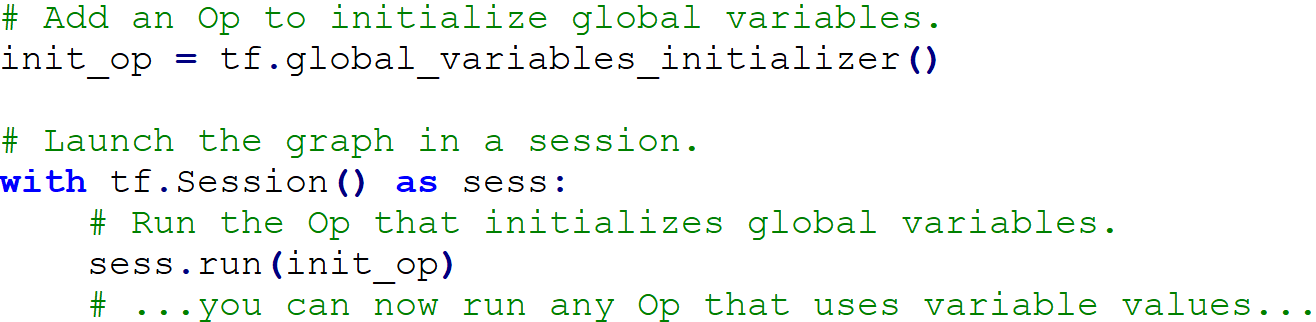
\includegraphics[width=0.95\textwidth]{img/tf/variable_initialization.png}
\end{tabular}
\end{figure}
\end{frame}

%%%%%%%%%%%%%%%%%%%%%%%%%%%%%%%%%%%%%%%%%%%%%%%%%%%%%%%%%%%%%%%%%%

\begin{frame}{Saving Variables}
Variables values can be saved with a \textbf{tf.train.Saver} object.
\begin{figure}
\begin{tabular}{c}
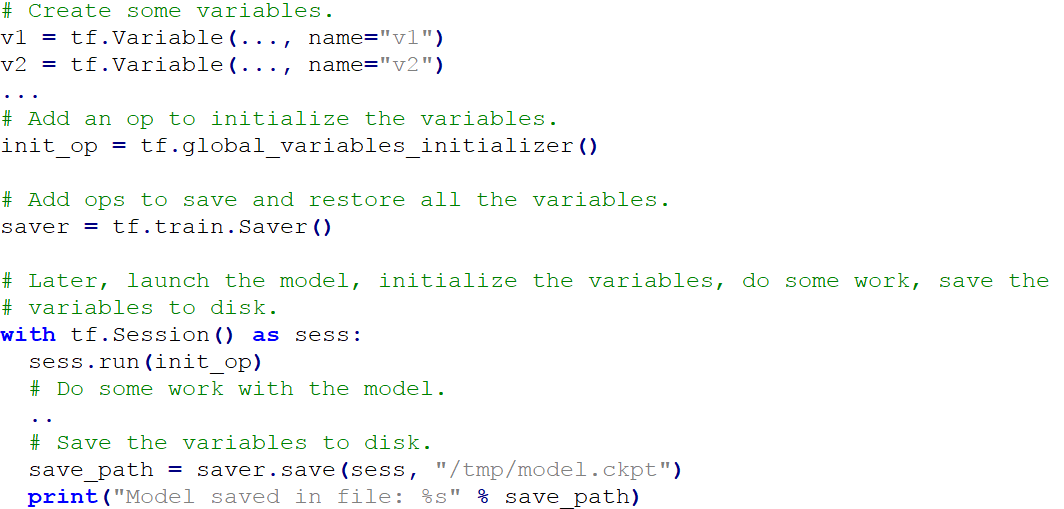
\includegraphics[width=0.8\textwidth]{img/tf/save_variables.png}
\end{tabular}
\end{figure}
\end{frame}

%%%%%%%%%%%%%%%%%%%%%%%%%%%%%%%%%%%%%%%%%%%%%%%%%%%%%%%%%%%%%%%%%%

\begin{frame}{Restoring Variables}
The same \textbf{tf.train.Saver} object can be used to restore variable values.
\begin{figure}
\begin{tabular}{c}
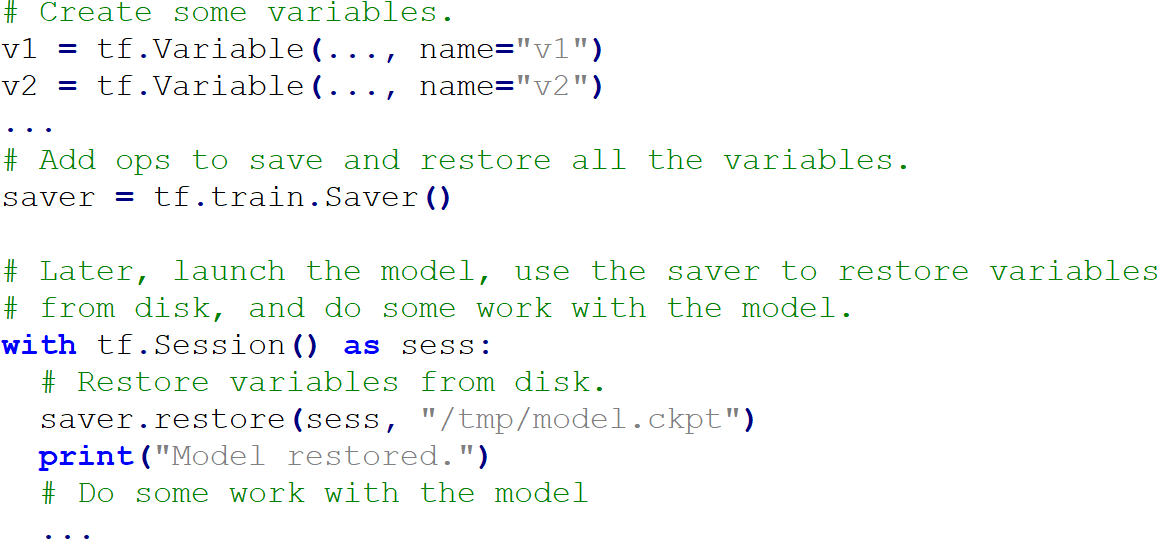
\includegraphics[width=0.8\textwidth]{img/tf/restore_variables.png}
\end{tabular}
\end{figure}
\end{frame}

%%%%%%%%%%%%%%%%%%%%%%%%%%%%%%%%%%%%%%%%%%%%%%%%%%%%%%%%%%%%%%%%%%

\begin{frame}{TensorBoard}
\textbf{TensorBoard} is a suite of visualization tools integrated with TensorFlow. You can use TensorBoard to visualize your TensorFlow graph, plot quantitative metrics about the execution of your graph, and show additional data like images that pass through it.
\begin{figure}
\begin{tabular}{c}
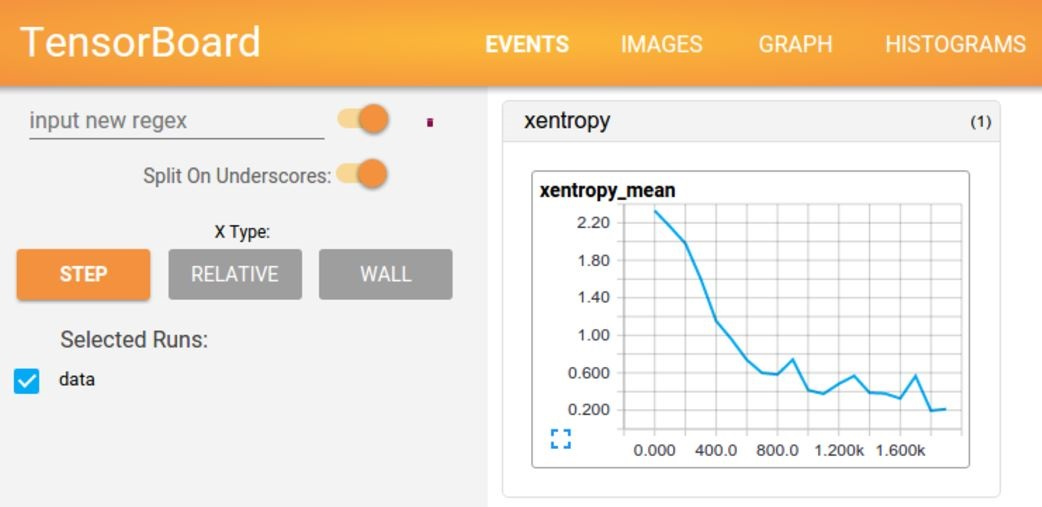
\includegraphics[width=0.7\textwidth]{img/tf/tensorboard.jpg}
\end{tabular}
\end{figure}
\end{frame}

%%%%%%%%%%%%%%%%%%%%%%%%%%%%%%%%%%%%%%%%%%%%%%%%%%%%%%%%%%%%%%%%%%

\begin{frame}{TensorBoard}
From a very high-level perspective, the lifecycle is the following:
\begin{itemize}
\item \textbf{tf.summary} operations can be attached to the nodes you'd like to collect summary data from.
\item \textbf{tf.summary.FileWriter} object is in charge of writing generated logs to a certain directory \texttt{logdir}
\item \textbf{TensorBoard} can be launched from command line as\\
\texttt{tensorboard --logdir=<logdir>}. TensorBoard is now available through your web browser at \texttt{localhost:6006}.
\end{itemize}
Official tutorial here: \url{https://www.tensorflow.org/get_started/summaries_and_tensorboard}
\end{frame}

%%%%%%%%%%%%%%%%%%%%%%%%%%%%%%%%%%%%%%%%%%%%%%%%%%%%%%%%%%%%%%%%%%
%%%%%%%%%%%%%%%%%%%%%%%%%%%%%%%%%%%%%%%%%%%%%%%%%%%%%%%%%%%%%%%%%%
%%%%%%%%%%%%%%%%%%%%%%%%%%%%%%%%%%%%%%%%%%%%%%%%%%%%%%%%%%%%%%%%%%

\section{References}

\begin{frame}[t, allowframebreaks]
\frametitle{References}
\bibliographystyle{abbrv}
\bibliography{bibliography}
\end{frame}

\end{document}